\section[Fully-coupled model]{Solving a problem using a Fully-Coupled Model}\label{tutorial-coupled}

The process of solving a problem using \Dumux can be roughly divided into four parts:
\begin{enumerate}
 \item The geometry of the problem and correspondingly a grid have to be defined.
 \item Material properties and constitutive relationships have to be selected.
 \item Boundary conditions as well as initial conditions have to be defined.
 \item A suitable model has to be chosen.
\end{enumerate}

The problem that is solved in this tutorial is illustrated in Figure \ref{tutorial-coupled:problemfigure}. A rectangular domain with no flow boundaries on the top and on the bottom which is initially saturated with oil is considered. Water infiltrates from the left side into the domain. Gravity effects as well as capillarity effects are neglected.

\begin{figure}[h]
\psfrag{x}{x}
\psfrag{y}{y}
\psfrag{no flow}{no flow}
\psfrag{water}{\textbf{water}}
\psfrag{oil}{\textcolor{white}{\textbf{oil}}}
\psfrag{p_w = 2 x 10^5 [Pa]}{$p_w = 2 \times 10^5$ [Pa]}
\psfrag{p_w_initial = 2 x 10^5 [Pa]}{\textcolor{white}{\textbf{$\mathbf{p_{w_{initial}} = 2 \times 10^5}$ [Pa]}}}
\psfrag{S_n = 0}{$S_n = 0$}
\psfrag{S_n_initial = 0}{\textcolor{white}{$\mathbf{S_{n_{initial}} = 1}$}}
\psfrag{q_w = 0 [kg/m^2s]}{$q_w = 0$ $\left[\frac{\textnormal{kg}}{\textnormal{m}^2 \textnormal{s}}\right]$}
\psfrag{q_n = -3 x 10^-4 [kg/m^2s]}{$q_n = -3 \times 10^{-2}$ $\left[\frac{\textnormal{kg}}{\textnormal{m}^2 \textnormal{s}}\right]$}
\centering
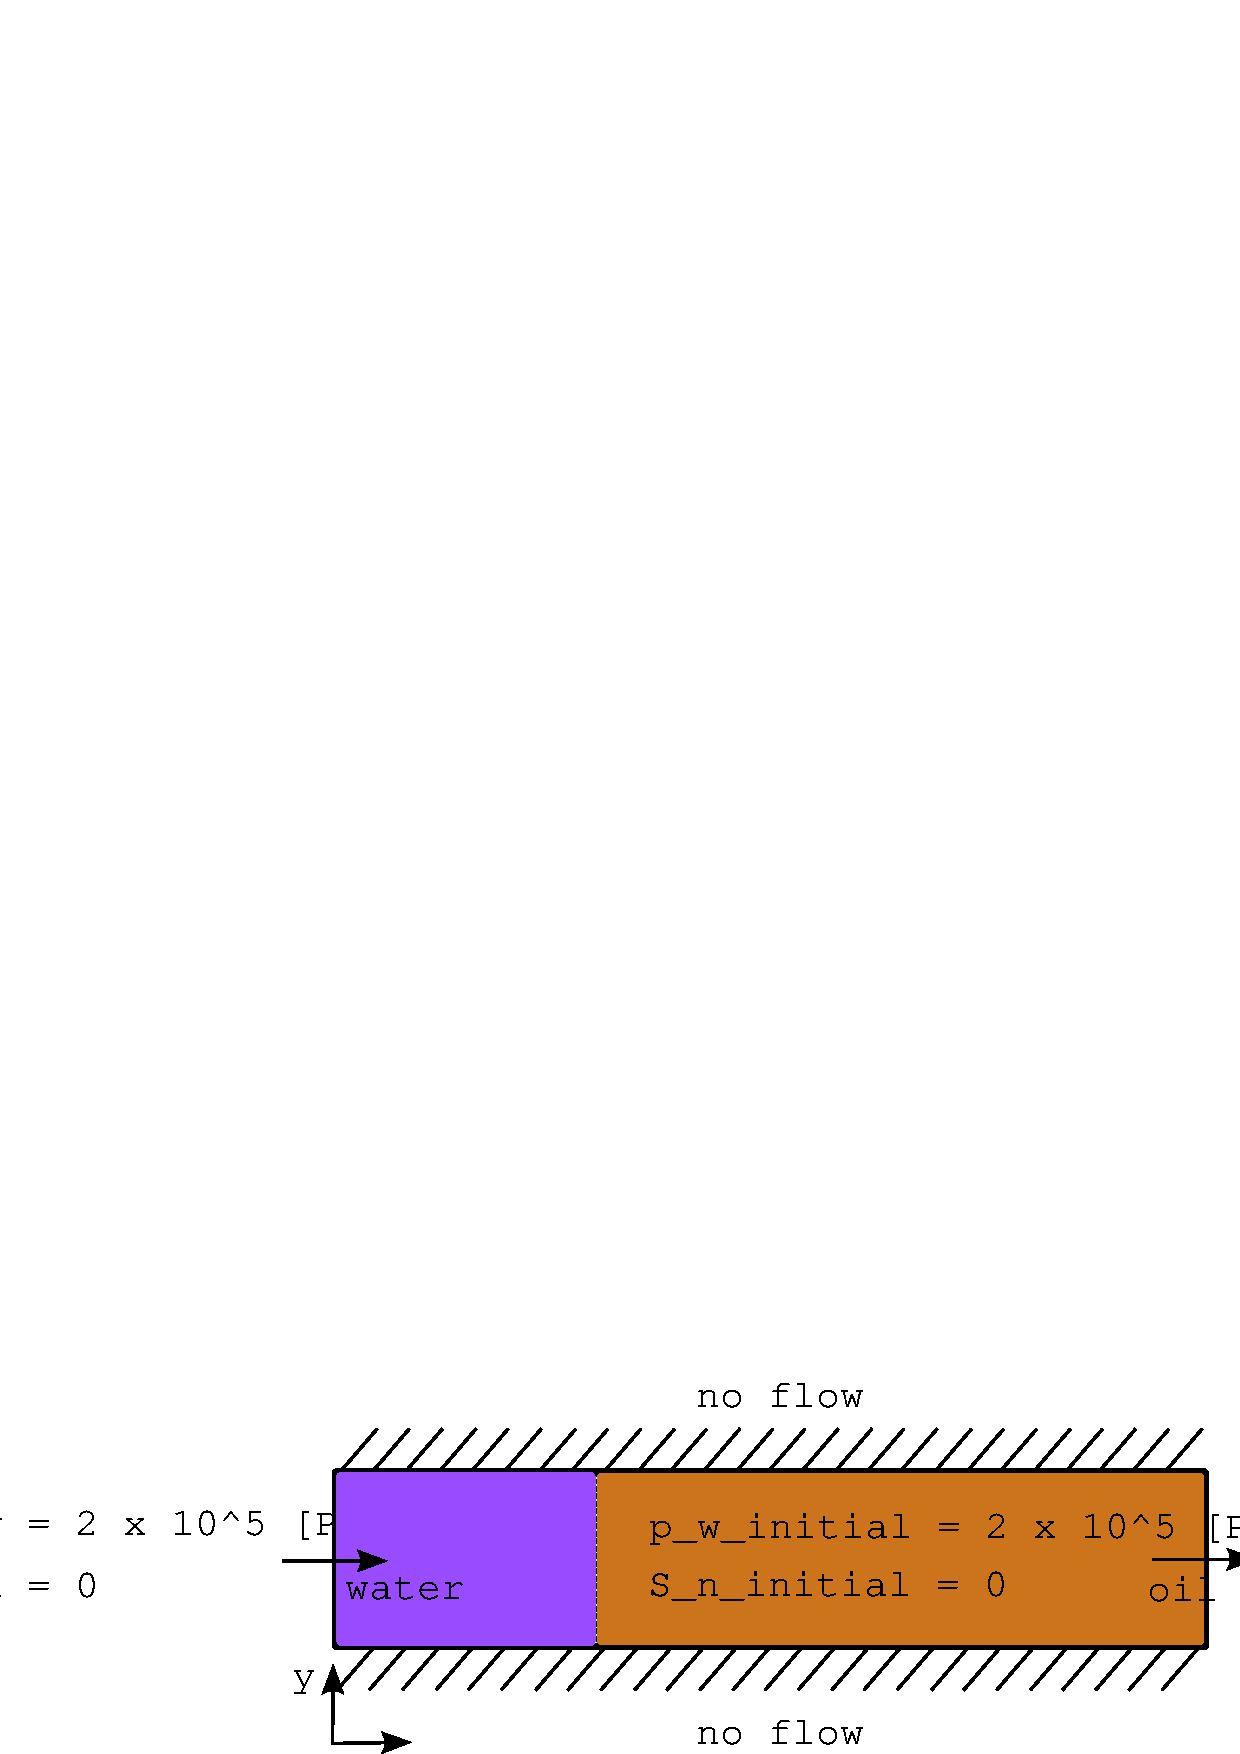
\includegraphics[width=0.9\linewidth,keepaspectratio]{EPS/tutorial-problemconfiguration}
\caption{Geometry of the tutorial problem with initial and boundary conditions.}\label{tutorial-coupled:problemfigure}
\end{figure}

The equations that are solved here are the mass balances of oil and
water:
\begin{align}
  \label{massbalancewater}
  \frac {\partial (\phi \, S_{w}\, \varrho_{w})}{\partial t}
  -
  \nabla \cdot \left( \varrho_{w} \, \frac{k_{rw}}{\mu_{w}} \, \mathbf{K}\;\nabla p_w \right)
  -
  q_w
  & =
  0 \\
  \label{massbalanceoil}
  \frac {\partial (\phi \, S_{o}\, \varrho_{o})}{\partial t}
  -
  \nabla \cdot \left( \varrho_{o} \, \frac{k_{ro}}{\mu_{o}} \, \mathbf{K}\;\nabla p_o \right)
  -
  q_o 
  & =
  0
\end{align}

\subsection{The main file}

Listing \ref{tutorial-coupled:mainfile} shows the main file
\texttt{tutorial/tutorial\_coupled.cc} for the coupled two-phase
model. This file needs to be executed to solve the problem described
above.

\begin{lst}[File tutorial/tutorial\_coupled.cc]\label{tutorial-coupled:mainfile} \mbox{}
  \lstinputlisting[basicstyle=\ttfamily\scriptsize,numbers=left,
  numberstyle=\tiny, numbersep=5pt, firstline=18]{../../tutorial/tutorial_coupled.cc}
\end{lst}

From line \ref{tutorial-coupled:include-begin} to line
\ref{tutorial-coupled:include-end} the \Dune and \Dumux files which
contain the needed functions and classes are included.

At line \ref{tutorial-coupled:set-type-tag} the type tag of the
problem which is going to be simulated is set. All other data types
can be retrieved by the \Dumux property system and only depend on this
single type tag. Retrieving them is done between line
\ref{tutorial-coupled:retrieve-types-begin} and
\ref{tutorial-coupled:retrieve-types-end}. For an introduction to the
property system, see section \ref{sec:propertysystem}.

The first thing which should be done at run time is to initialize the
message passing interface using \Dune's \texttt{MPIHelper} class. Line
\ref{tutorial-coupled:init-mpi} is essential if the simulation is
intended to be run on more than one processor at the same time. Next,
the command line arguments are parsed starting at line
\ref{tutorial-coupled:parse-args-begin} until line
\ref{tutorial-coupled:parse-args-end}. In this example, it is checked if and
from which time on a previous run of the simulation should be restarted. Furthermore, we
parse the time when the simulation ends and the initial time step size.

After this, a grid is created in line
\ref{tutorial-coupled:create-grid} and the problem is instantiated for
its leaf grid view in line \ref{tutorial-coupled:instantiate-problem}.
Finally, on line \ref{tutorial-coupled:begin-restart} a state written to
disk by a previous simulation run is restored if requested by the user.
The simulation procedure is started at line
\ref{tutorial-coupled:execute}.

\subsection{The problem class}

When solving a problem using \Dumux, the most important file is the
so-called \textit{problem file} as shown in listing
\ref{tutorial-coupled:problemfile} of
\texttt{tutorialproblem\_coupled.hh}.

\begin{lst}[File tutorial/tutorialproblem\_coupled.hh]\label{tutorial-coupled:problemfile} \mbox{}
\lstinputlisting[basicstyle=\ttfamily\scriptsize,numbers=left,
numberstyle=\tiny, numbersep=5pt, firstline=17]{../../tutorial/tutorialproblem_coupled.hh}
\end{lst}

First, a new type tag is created for the problem in line
\ref{tutorial-coupled:create-type-tag}.  In this case, the new type
tag inherits all properties defined for the \texttt{BoxTwoP} type tag,
which means that for this problem the two-phase box model is chosen as
discretization scheme. On line \ref{tutorial-coupled:set-problem}, a
problem class is attached to the new type tag, while the grid which
is going to be used is defined in line \ref{tutorial-coupled:set-grid} --
in this case that is  \texttt{SGrid}.  Since there's no uniform
mechanism to allocate grids in \Dune, the \texttt{Grid} property also contains
a static \texttt{create()} method which provides just that. Next,
the appropriate fluid system, that specifies both information about
the fluid mixture as well as about the pure substances, has to be chosen. 
The two-phase model defaults to the \texttt{FluidSystem2P} which assumes 
immiscibility of the phases, but requires that the wetting and non-wetting phases
are explicitly set. In this case, liquid water which uses the relations from 
IAPWS'97~\cite{IAPWS1997} is chosen as the wetting phase on line
\ref{tutorial-coupled:wettingPhase} and a liquid model oil is chosen as the 
non-wetting phase on line \ref{tutorial-coupled:nonwettingPhase}. 

For all parameters that depend on space, such as the properties of the
 soil, the specific spatial 
parameters for the problem of interest are specified in line
\ref{tutorial-coupled:set-spatialparameters}. The final property, which is set on line
\ref{tutorial-coupled:gravity}, is optional and tells the model not to
use gravity.

Parameters which are specific to a set-up -- like boundary and initial
conditions, source terms or temperature within the domain -- but are
required to solve the differential equations of the models are
specified via a \textit{problem} class. If the two-phase box model is
used, this class must be derived from \texttt{TwoPBoxProblem} as done
on line \ref{tutorial-coupled:def-problem}.

The problem class always has at least five methods:
\begin{itemize}
\item A method \texttt{boundaryTypes()} specifying the kind of
  boundary conditions to be used for a boundary segment
\item A method \texttt{dirichlet()} specifying the actual values for
  the Dirichlet conditions on a boundary segment
\item A method \texttt{neumann()} specifying the actual values for
  the Neumann conditions on a boundary segment
\item A method for source or sink terms called \texttt{source()}
\item A method called \texttt{initial()} for specifying the initial
  condition.
\end{itemize}

Methods which make statements about boundary segments of the grid (i.e. 
\texttt{boundaryTypes()}, \texttt{dirichlet()} and \texttt{neumann()}) get 
six parameters. The first parameter differs if the type of the boundary condition
is defined \texttt{boundaryTypes()}:
\begin{description}
\item[BCtypes:] A container which stores the type of the boundary condition
for each equation. For the typical case where all equations have the same boundary
condition at a certain position, there are two methods that set the appropriate conditions
for all primary variables / equations: Either \texttt{setAllDirichlet()} or \texttt{setAllNeumann()}.
\item[element:] The element of the grid where the boundary segment
  is located.
\item[fvElemGeometry:] The finite-volume geometry induced on the
  finite element by the box scheme.
\item[isIt:] The \texttt{IntersectionIterator} of the boundary
  segement as given by the grid
\item[scvIdx:] The index of the sub-control volume in
  \texttt{fvElementGeometry} adjacent to the boundary segment.
\item[boundaryFaceIdx:] The index of the boundary face in
  \texttt{fvElementGeometry} which represents the boundary segment.  
\end{description}
After the type of the boundary condition is defined, their values have to be
assigned with the methods \texttt{dirichlet()} and \texttt{neumann()} which only differ 
by the first function parameter:
\begin{description}
 \item[values:] A vector which stores the result of the method. What
  the values in this vector mean is dependent on the method: For
  \texttt{dirichlet()} it contains the values of the primary
  variables, for \texttt{neumann()} the mass fluxes per area unit
  over the boundary segment.
\end{description}

Similarly, the \texttt{initial()} and \texttt{source()} methods
specify properties of sub-control volumes and thus only get
\texttt{values}, \texttt{element}, \texttt{fvElemGeom} and
\texttt{scvIdx} as parameters.

In addition to these five methods, there might be some model-specific
methods. If the isothermal two-phase model is used, this includes 
for example a \texttt{temperature()} method which returns the temperature in Kelvin
of the fluids and the rock matrix in the domain. This temperature is
then used by the model to calculate fluid properties which possibly
depend on it, e.g. density.


\subsection{Defining fluid properties}\label{tutorial-coupled:description-fluid-class}

The \Dumux distribution includes some common substances which can be used
out of the box. The properties of the pure substances (such as the component 
nitrogen, water, or pseudo-component air) are stored in header files in 
the folder \verb+dumux/material/components+. Each of these files 
defines a class with the same name as the component but starting with a capital
letter, e.g. \texttt{Water}, and are derived from \texttt{Component}.

Most often, when two or more components are considered, fluid interactions 
such as solubility effects come into play and properties of mixtures such as 
the density are of interest. These interactions are defined in
a specific \verb+fluidsystem+ in the folder \verb+dumux/material/fluidsystems+.
It features methods returning fluid properties like density, enthalpy, viscosity,
etc. by accessing the pure components as well as binary coefficients such as
Henry or diffusion coefficients, which are stored in 
\verb+dumux/material/binarycoefficients+. New fluids which are not yet
 available in the \Dumux distribution can be defined analogously.

% In this example, a class for the definition of a two-phase system is used. This allows the choice 
% of the two components oil and water and to access the parameters that are relevant for the two-phase model.

\subsection{The definition of the parameters that are dependent on space}\label{tutorial-coupled:description-spatialParameters}

In \Dumux, the properties of the porous medium such as \textit{intrinsic 
permeability}, the \textit{porosity}, the \textit{heat capacity} as
well as the \textit{heat conductivity} can be defined in space using a
so-called \texttt{spatial parameters} class.  However, because the soil
also has an effect on the material laws of the fluids (e.g. \textit{capillarity}),
their selection and definition of their attributes (e.g. \textit{residual 
saturations}) are also accomplished in the spatial parameters.

The base class \texttt{Dumux::BoxSpatialParameters<TypeTag>} holds a general 
averaging procedure for vertex-centered box-methods.

Listing \ref{tutorial-coupled:spatialparametersfile} shows the file
\verb+tutorialspatialparameters_coupled.hh+:

\begin{lst}[File tutorial/tutorialspatialparameters\_coupled.hh]\label{tutorial-coupled:spatialparametersfile} \mbox{}
\lstinputlisting[basicstyle=\ttfamily\scriptsize,numbers=left,
numberstyle=\tiny, numbersep=5pt, firstline=16]{../../tutorial/tutorialspatialparameters_coupled.hh}
\end{lst}

First, a certain material law that best describes the problem at hand has to
be selected in line \ref{tutorial-coupled:rawlaw}\label{tutorial-coupled:materialLaw}. 
\Dumux provides several material laws in the folder 
\verb+dumux/material/fluidmatrixinteractions+.
The selected one -- here it is a relation according to a regularized version of Brooks \& Corey --  is included
in line \ref{tutorial-coupled:rawLawInclude}. After the selection,
an adapter in line \ref{tutorial-coupled:eff2abs} translates between the law
for effective values (the Brooks \& Corey model) and the saturations generated as simulations results, i.e. residual saturations are considered. 
As the applied raw law knows best which kind of parameters are necessary,
it provides a parameter class \texttt{RegularizedBrooksCoreyParams} that is
accessible via the member \texttt{Params} and defined in line 
\ref{tutorial-coupled:matLawObjectType}. The material law object 
is now instantiated correctly as a private object
in line \ref{tutorial-coupled:matParamsObject}.

In line \ref{tutorial-coupled:permeability} the function returning the
intrinsic permeability can be found. As can be seen, the function has
to be called with three different arguments. 
(\texttt{Element}) is again the current element, which also holds information
about its geometry and position, the second argument
(\texttt{fvElemGeom}) holds information about the finite-volume geometry induced
by the box-method, and the third defines the index of the current sub-control 
volume. The intrinsic permeability is a tensor and is thus returned in form of
a $\texttt{dim} \times \texttt{dim}$-matrix where \texttt{dim} is the dimension 
of the problem. 

The function \texttt{porosity()} defined in line
\ref{tutorial-coupled:porosity} is called with the same arguments as
the permeability function described before and returns the porosity
dependent on the position in the domain.

Next, the method \texttt{materialLawParams()} defines in line 
\ref{tutorial-coupled:matLawParams} which \verb+materialLawParams+ object 
 should be applied at this specific position. Although in this case only one objects is returned, 
in general the problem may be heterogeneous, demanding for different objects at different positions in space. 
While the selection of the type of this object was already explained (line \ref{tutorial-coupled:rawLawInclude}),
 some specific parameter 
values of the applied material law are still needed. This is 
done in the constructor body (line \ref{tutorial-coupled:setLawParams}).
Depending on the type of the \texttt{materialLaw} object, the adequate \texttt{set}-methods
are provided by the object to access all necessary parameters 
for the applied material law. The name of the access / set functions as well as the rest of the implementation 
of the material description can be found in 
\verb+dumux/dumux/material/fluidmatrixinteractions/2p+.

\subsection{Exercises}
\label{tutorial-coupled:exercises}
The following exercises will give you the opportunity to learn how you
can change soil parameters, boundary conditions and fluid properties
in \Dumux. For each exercise you can find the output file of the last
timestep in the directory \texttt{tutorial/results/coupled}.

\subsubsection{Exercise 1}
\renewcommand{\labelenumi}{\alph{enumi})} For Exercise 1 you only have
to make some small changes in the tutorial files.  

\begin{enumerate}

\item \textbf{Run the Model} \\
To get an impression what the results should look like you can first run the original version of the coupled tutorial model by typing  \texttt{./tutorial\_coupled 5e5 10}. The first number behind the simulation name defines the timespan of the simulation run in seconds, the second number defines the initial time step size. Note that the time step size is automatically optimized during the simulation. For the visualisation with paraview please refer to \ref{quick-start-guide}.\\

\item \textbf{Changing the Model Domain and the Boundary Conditions} \\
  Change the size of the model domain so that you get a rectangle with
  edge lengths of $\text{x} = 400 m$ and $\text{y} = 500 m$ and with
  discretization lengths of $\Delta \text{x} = 20$ m and $\Delta
  \text{y} = 20$ m.
  
  Change the boundary conditions in the file
  \texttt{tutorialproblem\_coupled.hh} so that water enters from the
  bottom and oil is extracted from the top boundary. The right and the
  left boundary should be closed for water and oil fluxes. 

  Compile the main file by typing \texttt{make tutorial\_coupled} and
  run the model.


\item \textbf{Changing Fluids} \\
  Now you can change the fluids. Use \texttt{DNAPL} instead of
  \texttt{Oil} and \texttt{Brine} instead of \texttt{Water}. To do
  that you have to change the problem file:
  \begin{enumerate}
  \item Brine: The class \texttt{Dumux::Brine} acts as an adapter to pure water. Hence, it needs not only \texttt{<Scalar>} as a template argument, but also the complete water class used before (be aware to use the water class with its own template parameters).
 \item DNAPL: A standard set of chemical substances represented by the class \texttt{Dumux::SimpleDNAPL} is located in the folder \texttt{dumux/material/components/} and needs to be included in the problem file.
\end{enumerate}
  If you want to take a closer look how the fluid classes are defined 
  and which substances are already available please browse through the files in the directory
  \texttt{/dumux/material/components}.

\item \textbf{Use the \Dumux fluid system} \\
\Dumux usually organises fluid mixtures via a \texttt{fluidsystem}. In order to include a fluidsystem you first have to comment the lines \ref{tutorial-coupled:2p-system-start} to \ref{tutorial-coupled:2p-system-end} in the problem file. If you use eclipse, this can easily be done by pressing \textit{str + shift + 7} -- the same as to cancel the comment later on.\\
Now include the file \texttt{fluidsystems/h2o\_n2\_system.hh} in the material folder, and set a property \texttt{FluidSystem} with the appropriate type, \texttt{Dumux::H2O\_N2\_System<TypeTag>}. However, the complicated fluidsystem uses tabularized fluid data, which need to be initilized in the constructor body of the current problem by adding \texttt{GET\_PROP\_TYPE(TypeTag, PTAG(FluidSystem))::init();}, hence using the initialization function of the applied fluidsystem. As water flow replacing a gas is much faster, test your simulation only until 2e3 seconds and start with a time step of 1 second.\\
Please reverse the changes of this example, as we still use bulk phases and hence do not need such an extensive fluid system.

\item \textbf{Changing Constitutive Relations} \\
  Use an unregularized linear law with an entry pressure of $p_e = 0.0$ and maximal capillary pressure of e.g. $p_{c_{max}} = 2000.0$ instead of using a
 regularized Brooks-Corey law for the
  relative permeability and for the capillary pressure saturation relationship. To do that you have
  to change the file \texttt{tutorialspatialparameters\_coupled.hh}. 
 You can find the material laws in the folder 
  \verb+dumux/material/fluidmatrixinteractions+. The necessary parameters
of the linear law and the respective \texttt{set}-functions can be found
 in the file \\
 \verb+dumux/material/fluidmatrixinteractions/2p/linearmaterialparams.hh+.
 
\item \textbf{Heterogeneities}  \\
  Set up a model domain with the soil properties given in Figure
  \ref{tutorial-coupled:exercise1_d}. Adjust the boundary conditions
  so that water is again flowing from the left to the right of the
\begin{figure}[h]
\psfrag{K1 =}{K $= 10^{-8}\text{ m}^2$}
\psfrag{phi1 =}{$\phi = 0.15$}
\psfrag{K2 =}{\textcolor{white}{K $= 10^{-9}\text{ m}^2$}}
\psfrag{phi2 =}{\textcolor{white}{$\phi = 0.3$}}
\psfrag{600 m}{600 m}
\psfrag{300 m}{300 m}
\centering
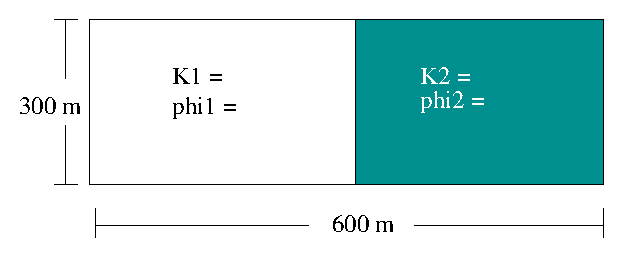
\includegraphics[width=0.5\linewidth,keepaspectratio]{EPS/exercise1_c.eps}
\caption{Exercise 1f: Set-up of a model domain with a heterogeneity. $\Delta \text{x} = 20$ m $\Delta \text{y} = 20$ m.}\label{tutorial-coupled:exercise1_d}
\end{figure}
domain. You can use the fluids of exercise 1c). 
When does the front cross the material border? In paraview, the option \textit{View} $\rightarrow$ \textit{Animation View} is nice to get a rough feeling of the timestep sizes.
\end{enumerate}

\subsubsection{Exercise 2}
For this exercise you should create a new proplem file analogous to
the file \texttt{tutorialproblem\_coupled.hh} and new spatial parameters 
just like \texttt{tutorialspatialparameters\_coupled.hh}. The new problem file needs to
be included in the file \texttt{tutorial\_coupled.cc}.  \\
The new file defining spatial parameters should contain the definition 
of a new class, such as \\
\texttt{SpatialParametersEx2}. Make sure that you also adjust the guardian
macros in the header files (e.g. change \\
\texttt{TUTORIALSPATIALPARAMETERS\_COUPLED} to
\texttt{SPATIALPARAMETERSEX2}). Besides also adjusting the guardian macros, 
the new problem file should define and use a new type tag for the problem as well as a new problem class
e.g. \texttt{ProblemEx2}. Make sure you assign your newly defined spatial 
parameter class to the \texttt{SpatialParameters} property for the new 
type tag. \\
After this, change the \texttt{create()} method of the \texttt{Grid}
property so that it matches the domain described
by figure \ref{tutorial-coupled:ex2_Domain}. Adapt the problem class
so that the boundary conditions are consistent with figure
\ref{tutorial-coupled:ex2_BC}. Initially the domain is fully saturated
with water and the pressure is $p_w = 5 \times 10^5 \text{Pa}$. Oil
infiltrates from the left side. Create a grid with $20$ cells in
$x$-direction and $10$ cells in $y$-direction. The simulation time
should be set to $1\times 10^6 \text{ s}$ with an initial time step size of
$100 \text{ s}$.

Now include your new problem file in the main file and replace the
\texttt{TutorialProblemCoupled} type tag by the one you've created and
compile the program.


\begin{figure}[h]
\psfrag{K1}{K $= 10^{-7}\text{ m}^2$}
\psfrag{phi1}{$\phi = 0.2$}
\psfrag{Lin}{Brooks-Corey Law}
\psfrag{Lin2}{$\lambda = 1.8$, $p_e = 1000$}
\psfrag{K2}{K $= 10^{-9}\text{ m}^2$}
\psfrag{phi2}{$\phi = 0.15$}
\psfrag{BC1}{Brooks-Corey Law} 
\psfrag{BC2}{$\lambda = 2$, $p_e = 1500$}
\psfrag{H1y}{50 m}
\psfrag{H2y}{15 m}
\psfrag{H3y}{20 m}
\psfrag{L1x}{100 m}
\psfrag{L2x}{50 m}
\psfrag{L3x}{25 m}
\centering
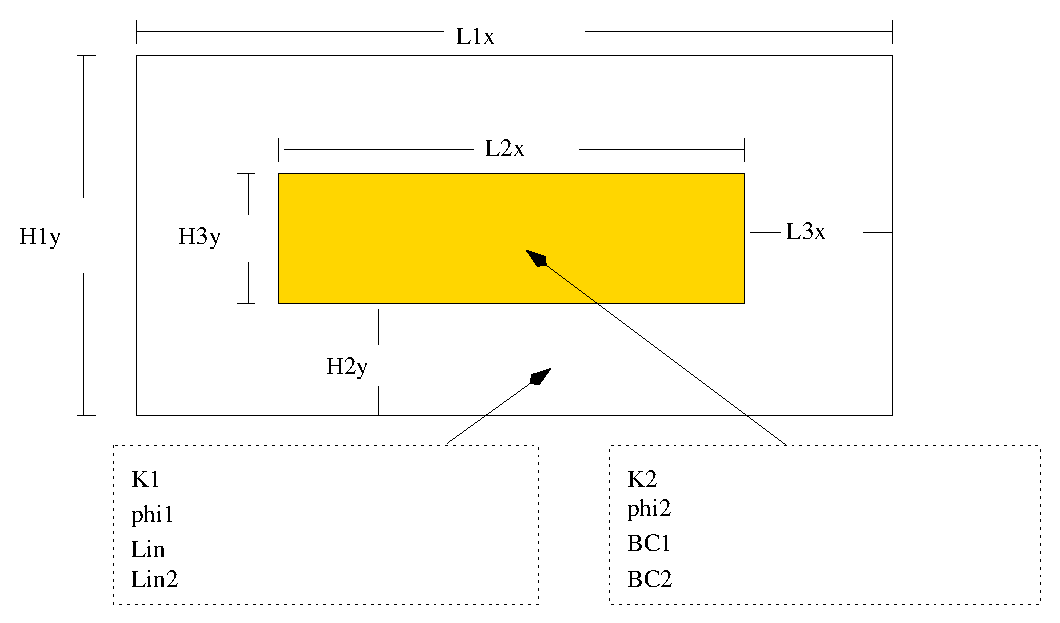
\includegraphics[width=0.8\linewidth,keepaspectratio]{EPS/Ex2_Domain.eps}
\caption{Set-up of the model domain and the soil parameters}\label{tutorial-coupled:ex2_Domain}
\end{figure}

\begin{figure}[h]
\psfrag{pw}{$p_w = 5 \times 10^5$ [\text{Pa}]}
\psfrag{S}{$S_n = 1.0$}
\psfrag{qw}{$q_w = 2 \times 10^{-4}$ [kg/$\text{m}^2$s]}
\psfrag{qo}{$q_n = 0.0$ [kg/$\text{m}^2$s]}
\psfrag{no flow}{no flow}
\centering
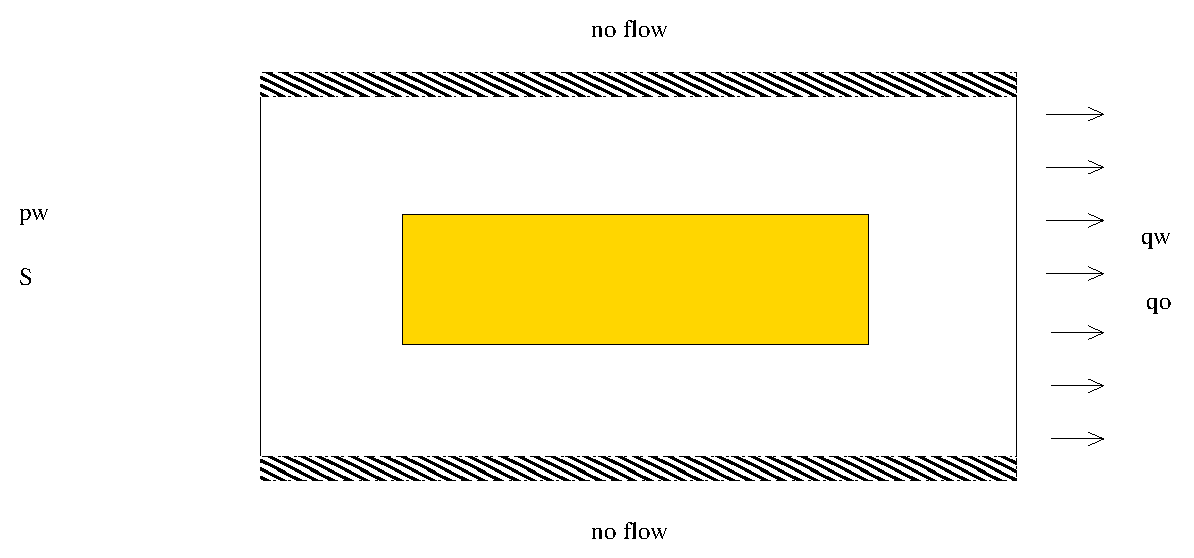
\includegraphics[width=0.8\linewidth,keepaspectratio]{EPS/Ex2_Boundary.eps}
\caption{Boundary Conditions}\label{tutorial-coupled:ex2_BC}
\end{figure}

\begin{itemize}
 \item Increase the simulation time to e.g. $4\times 10^7 \text{ s}$. Investigate the saturation: Is the value range reasonable?
 \item What happens if you increase the resolution of the grid?
\end{itemize}

\subsubsection{Exercise 3}

Create a new file for benzene called \texttt{benzene.hh} and implement
a new fluid system. (You may get a hint by looking at existing fluid 
systems in the directory \verb+/dumux/material/fluidsystems+.) \\
Use benzene as a new fluid and run the model of Exercise 2 with water
and benzene. Benzene has a density of $889.51 \, \text{kg} / \text{m}^3$
and a viscosity of $0.00112 \, \text{Pa} \; \text{s}$. 


%%% Local Variables: 
%%% mode: latex
%%% TeX-master: "dumux-handbook"
%%% End: 
